\section{Experiments}
In this section, we present three experiments conducted to evaluate the performance of pretrained models on depth images. First, we establish a baseline by comparing model accuracy across different colormaps applied to the depth images. Second, we explore the impact of fine-tuning on model performance using the stacked colormap representation. Finally, we assess the models on subsets of ImageNet and the Washington RGB-D dataset to understand their behavior on tasks with reduced label spaces and lower complexity.

\subsection{ImageNet 1k-class Depth}
We initiated our experiments by evaluating the performance of the models ``as-is'', without any fine-tuning applied to the depth images.

The models employed in this study (AlexNet, VGG19, InceptionV3, ResNet50) were conveniently pretrained on the same 1,000 classes as our dataset. This alignment was achieved by carefully curating the dataset, thereby obviating the need to fine-tune the final layer of the classifier, as it already produced the correct labels.

To establish a baseline and investigate whether the models exhibited varying performance under different colormaps of the depth images, we experimented with a stacked approach, grayscale, viridis, plasma and magma colormaps as shown in \autoref{fig:model_acc_by_colormap} and summarized in \autoref{tab:baseline_accuracy}.

\begin{figure}[h]
    \centering
    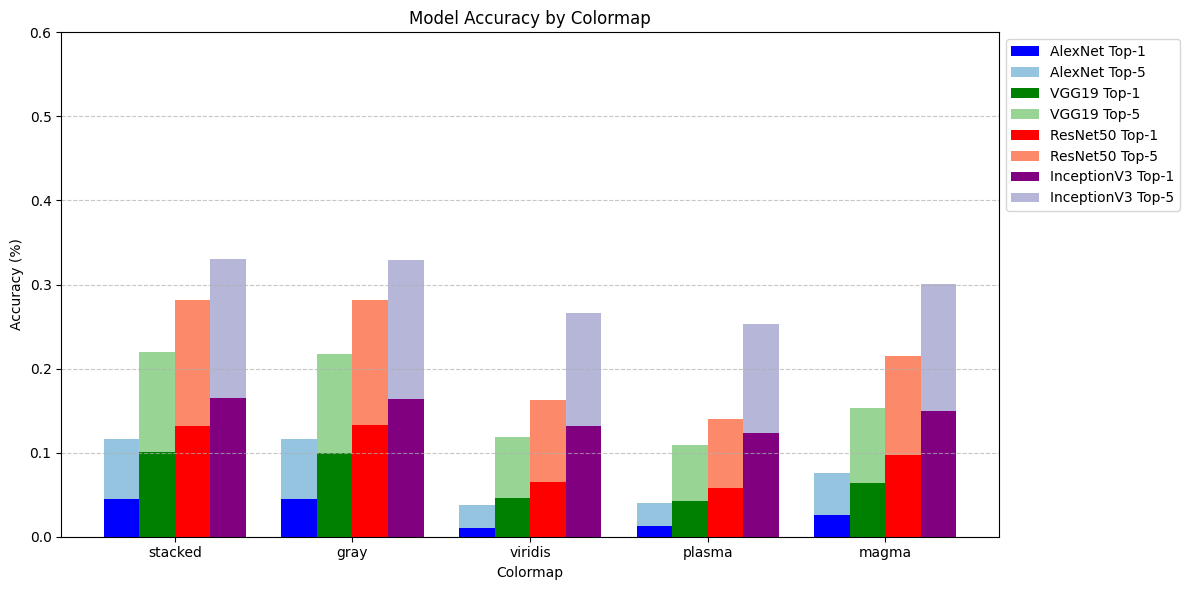
\includegraphics[width=1\linewidth]{./images/model_acc_by_colormap.png}
    \caption{Baseline accuracy comparison across colormaps for ImageNet 1k-class depth.}
    \label{fig:model_acc_by_colormap}
\end{figure}

\begin{table*}[htbp]
    \centering
    \begin{tabular}{|l|c|c|c|c|c|c|c|c|c|c|c|c|}
        \hline
        \multirow{2}{*}{Model} & \multicolumn{2}{|c|}{Stacked} & \multicolumn{2}{|c|}{Grayscale} & \multicolumn{2}{|c|}{Viridis} & \multicolumn{2}{|c|}{Plasma} & \multicolumn{2}{|c|}{Magma} \\
        \cline{2-11}
         & Top-1 & Top-5 & Top-1 & Top-5 & Top-1 & Top-5 & Top-1 & Top-5 & Top-1 & Top-5 \\
        \hline
        AlexNet & \textbf{04.53} & \textbf{11.63} & 04.50 & 11.62 & 01.04 & 03.83 & 01.24 & 03.98 & 02.54 & 07.59 \\
        \hline
        VGG19 & \textbf{10.04} & \textbf{22.00} & 09.97 & 21.79 & 04.64 & 11.87 & 04.29 & 10.95 & 06.45 & 15.31 \\
        \hline
        ResNet50 & 13.18 & \textbf{28.16} & \textbf{13.27} & 28.16 & 06.56 & 16.23 & 05.83 & 14.00 & 09.71 & 21.44 \\
        \hline
        InceptionV3 & \textbf{16.48} & \textbf{33.05} & 16.40 & 32.94 & 13.16 & 26.66 & 12.36 & 25.34 & 15.01 & 30.07 \\
        \hline
    \end{tabular}
    \caption{Baseline accuracy comparison across colormaps for ImageNet 1k-class depth.}
    \label{tab:baseline_accuracy}
\end{table*}

\begin{table*}[htbp]
    \centering
    \begin{tabular}{|l|cc|cc|cc|}
        \hline
        \multicolumn{1}{|c|}{\multirow{2}{*}{Model}} & \multicolumn{2}{c|}{Baseline} & \multicolumn{2}{c|}{Partial Fine-Tuning} & \multicolumn{2}{c|}{Fine-Tuning}                                 \\ \cline{2-7} 
        \multicolumn{1}{|c|}{}                       & \multicolumn{1}{c|}{Top-1}  & Top-5 & \multicolumn{1}{c|}{Top-1}    & Top-5    & \multicolumn{1}{c|}{Top-1}                & Top-5                \\ \hline
        AlexNet                                      & \multicolumn{1}{c|}{04.53}  & 11.63 & \multicolumn{1}{c|}{18.05}    & 36.41    & \multicolumn{1}{c|}{\textbf{23.62}}       & \textbf{45.76}       \\ \hline
        VGG19                                        & \multicolumn{1}{c|}{10.04}  & 22.00 & \multicolumn{1}{c|}{25.40}    & 48.18    & \multicolumn{1}{c|}{\textbf{34.20}}       & \textbf{60.96}       \\ \hline
        ResNet50                                     & \multicolumn{1}{c|}{13.18}  & 28.16 & \multicolumn{1}{c|}{32.36}    & 57.87    & \multicolumn{1}{c|}{\textbf{44.95}}       & \textbf{71.90}       \\ \hline
        InceptionV3                                  & \multicolumn{1}{c|}{16.48}  & 33.05 & \multicolumn{1}{c|}{22.31}    & 44.57    & \multicolumn{1}{c|}{\underline{\textbf{48.53}}} & \underline{\textbf{74.53}} \\ \hline
    \end{tabular}
    \caption{Fine-tuning accuracy comparison for ImageNet 1k-class depth.}
    \label{tab:finetuning_accuracy}
\end{table*}

This experiment demonstrated that the grayscale approach yielded results most familiar to the models. Furthermore, we established that a straightforward approach, such as duplicating the original single-channel depth image to the three channels required by these models, is as robust as applying a colormap function to the grayscale image.

Further experimentation involving fine-tuning these models resulted in a significant increase in accuracy. Given the strong performance of the "stacked" colormap, we focused on this approach for fine-tuning and excluded other colormaps from further analysis.

The partial fine-tuning procedure involved freezing all model parameters except for a small subset of layers that were specifically selected for training. In the case of \textbf{AlexNet}, only the final \texttt{classifier} layer was unfrozen and trained. For \textbf{VGG19}, we applied the same strategy, unfreezing only the \texttt{classifier} module. In the case of \textbf{ResNet50}, we unfroze both the last residual block (\texttt{layer 4}) and the final fully connected layer (\texttt{layer 5}). Finally, for \textbf{InceptionV3}, the fine-tuning was performed by unfreezing the last inception block (\texttt{Mixed\_7c}), the auxiliary classifier (\texttt{AuxLogits}), and the final fully connected layer (layer 5).

The complete fine-tuning procedure involved unfreezing all model parameters, allowing the models to adapt fully to the depth images. This approach was computationally more expensive but yielded higher accuracy.

As reported in \autoref{tab:finetuning_accuracy}, both partial and complete fine-tuning substantially improved model performance on depth images. The stacked colormap representation proved effective, with InceptionV3 achieving the highest Top-1 accuracy (48.53\%) and Top-5 accuracy (74.53\%). These results suggest that models originally developed for RGB image classification retain their relative performance ranking when applied to depth data. For instance, architectures that achieve higher accuracy on RGB tasks (e.g., InceptionV3 vs. AlexNet) also perform better on depth images, indicating that the improvements are architecture-driven rather than modality-specific.

While both fine-tuning strategies enhanced the models' ability to interpret depth images, the limited number of examples per class in our dataset constrained the overall performance. Nonetheless, the improvements observed with complete fine-tuning are notable: on average, we recorded a nearly \textbf{3x} increase in accuracy compared to the baseline (computed as the mean ratio between complete fine-tuning and baseline results for Top-1 and Top-5 across all models). 
% This supports further exploration in this direction.

\subsection{ImageNet Subset (200 Classes)}

As shown in \autoref{tab:imagenet_subset_accuracy}, complete fine-tuning consistently outperforms partial fine-tuning across all models on the 200-class subset. InceptionV3 achieves the highest Top-1 accuracy (47.95\%, 72.80\% ), while ResNet50 leads in Top-5 accuracy (47.75\%, 73.20\%). The relative performance ranking of the models aligns with the results from the 1000-class subset, indicating stable model behavior despite the smaller dataset size. Both fine-tuning approaches improve performance; however, deeper networks benefit more substantially from complete fine-tuning, highlighting the importance of end-to-end adaptation when working with limited data.

\begin{table*}[htbp]
    \centering
    \begin{minipage}[t]{0.48\textwidth}
        \centering
        \begin{tabular}{|l|c|c|c|c|}
            \hline
            \multirow{2}{*}{Model} & \multicolumn{2}{|c|}{Partial FT} & \multicolumn{2}{|c|}{Complete FT} \\ \cline{2-5}
             & Top-1 & Top-5 & Top-1 & Top-5 \\
            \hline
            AlexNet & 26.25 & \textbf{52.90} & \textbf{26.40} & 51.25 \\
            \hline
            VGG19 & 32.50 & 59.95 & \textbf{36.70} & \textbf{65.25} \\
            \hline
            ResNet50 & 44.30 & 71.15 & \textbf{47.75} & \textbf{73.20} \\
            \hline
            InceptionV3 & 38.70 & 64.15 & \textbf{47.95} & \textbf{72.80} \\
            \hline
        \end{tabular}
        \caption{Accuracy on 200-class ImageNet subset.}
        \label{tab:imagenet_subset_accuracy}
    \end{minipage}
    \hfill
    \begin{minipage}[t]{0.48\textwidth}
        \centering
        \begin{tabular}{|l|c|c|}
            \hline
            Model & Top-1 & Top-5 \\
            \hline
            AlexNet & 87.51 & 98.79 \\
            \hline
            VGG19 & 92.23 & 99.61 \\
            \hline
            ResNet50 & 88.48 & 99.31 \\
            \hline
            InceptionV3 & 89.45 & 99.08 \\
            \hline
        \end{tabular}
        \caption{Partial fine-tuning accuracy on Washington RGB-D.}
        \label{tab:washington_rgbd_accuracy}
    \end{minipage}
\end{table*}

\subsection{Washington RGB-D Dataset}
Following the same approach we used again the stacked colormap representation for the Washington RGB-D dataset. In contrast, the Washington RGB-D dataset comprises only 51 classes, with an average of 821 images per class, unlike ImageNet, which has only 50, representing a significantly lower task complexity and substantially larger training data. 

As reported in \autoref{tab:washington_rgbd_accuracy}, all models achieved near 90\% Top-1 accuracy, with VGG19 reaching up to 92.23\%. These results were obtained using partial fine-tuning alone. Given this high baseline, we opted not to undertake complete fine-tuning, concluding that the incremental improvements would not justify the higher computational expense. 

Overall, for sufficiently large datasets, transfer learning tends to be highly effective, eliminating the need for complete fine-tuning.
